% Agent–Environment interaction diagram – PPT colour scheme
% Compile: xelatex agent_environment_tikz.tex
% Convert: pdf2svg agent_environment_tikz.pdf agent_environment_tikz.svg
\documentclass[border=10pt]{standalone}
\usepackage{fontspec}
\setmainfont{Aptos}[
  Path = /Applications/Microsoft Word.app/Contents/Resources/DFonts/,
  Extension = .ttf,
  UprightFont = Aptos,
  BoldFont = Aptos-Bold,
  ItalicFont = Aptos-Italic,
  BoldItalicFont = Aptos-Bold-Italic,
]
\usepackage{amsmath,amssymb}
\usepackage{tikz}
\usetikzlibrary{arrows.meta, calc}

% PPT colours
\definecolor{accent}{HTML}{CB8044}
\definecolor{fg}{HTML}{E8E8E8}
\definecolor{fgdim}{HTML}{AAAAAA}
% Robot colours
\definecolor{robotdark}{HTML}{2A2A2A}
\definecolor{robotmid}{HTML}{3D3D3D}
% Globe colours
\definecolor{land}{HTML}{7BA656}       % visible green for land
\definecolor{ocean}{HTML}{5C85A8}      % blue for oceans

\begin{document}
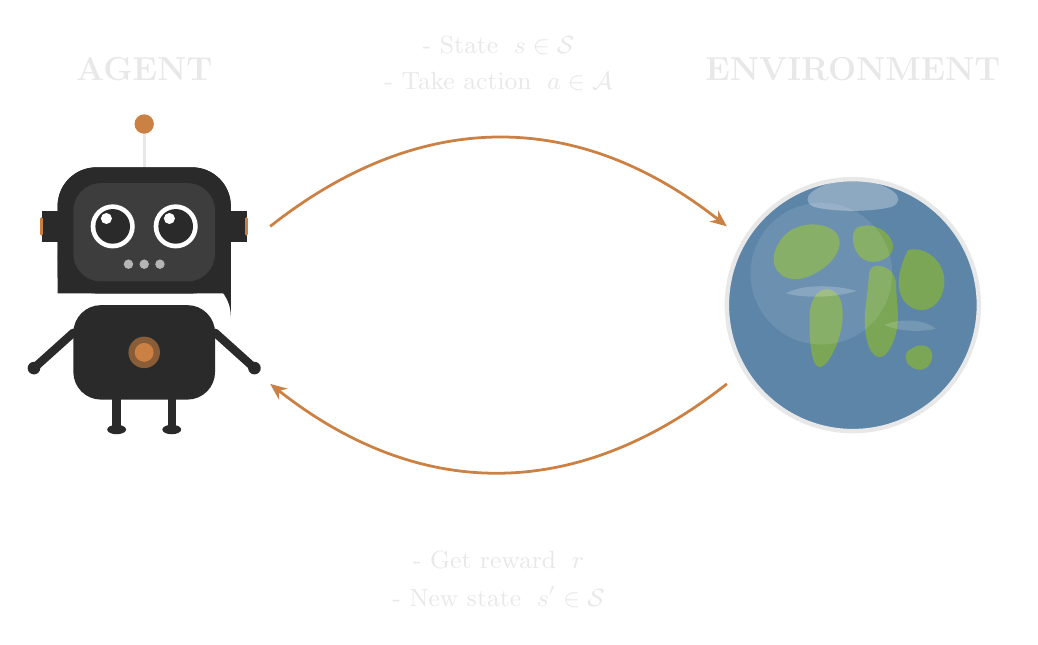
\begin{tikzpicture}[
    >=Stealth,
    curvedarrow/.style={
        accent,
        line width=1pt,
        -{Stealth[length=6pt, width=5pt]},
    },
]

% =============================================
% AGENT – Cute robot (inspired by the original PNG)
% Centred at (0, 0.5)
% =============================================
\begin{scope}[shift={(0,0.3)}, line cap=round, line join=round]

  % --- Antenna ---
  \draw[fg, line width=1.2pt] (0,1.95) -- (0,2.45);
  \fill[accent] (0,2.5) circle (3.5pt);

  % --- Head: rounded rectangle, dark filled ---
  \fill[robotdark] (-1.1,0.35) [rounded corners=14pt] -- (-1.1,1.95) -- (1.1,1.95) [rounded corners=0pt] -- (1.1,0.35) -- cycle;
  \fill[robotdark] (-1.1,0.35) [rounded corners=0pt] -- (-1.1,0.55) [rounded corners=14pt] -- (1.1,0.55) -- (1.1,0.35) -- cycle;
  % Simpler: just one rounded rect
  \path[fill=robotdark, rounded corners=14pt] (-1.1,0.35) rectangle (1.1,1.95);

  % --- White face area (visor-like but rectangular, not a helmet) ---
  % Just a lighter inset area for the face
  \path[fill=robotmid, rounded corners=10pt] (-0.9,0.5) rectangle (0.9,1.75);

  % --- Eyes: large, round, dark with white reflection ---
  % Like the original: big dark circles with a white crescent
  % Left eye
  \fill[white] (-0.4,1.2) circle (0.28);
  \fill[robotdark] (-0.4,1.2) circle (0.22);
  \fill[white] (-0.48,1.3) circle (0.07);
  % Right eye
  \fill[white] (0.4,1.2) circle (0.28);
  \fill[robotdark] (0.4,1.2) circle (0.22);
  \fill[white] (0.32,1.3) circle (0.07);

  % --- Mouth: three dots (like the original PNG) ---
  \fill[fg, opacity=0.7] (-0.2,0.72) circle (0.06);
  \fill[fg, opacity=0.7] (0.0,0.72) circle (0.06);
  \fill[fg, opacity=0.7] (0.2,0.72) circle (0.06);

  % --- Ears (small rectangles on sides of head) ---
  \fill[robotdark] (-1.1,1.0) rectangle (-1.3,1.4);
  \draw[accent, line width=1pt] (-1.3,1.1) -- (-1.3,1.3);
  \fill[robotdark] (1.1,1.0) rectangle (1.3,1.4);
  \draw[accent, line width=1pt] (1.3,1.1) -- (1.3,1.3);

  % --- Body: rounded rectangle, slightly narrower than head ---
  \path[fill=robotdark, rounded corners=10pt] (-0.9,-1.0) rectangle (0.9,0.2);
  % Body accent circle
  \fill[accent, opacity=0.6] (0,-0.4) circle (0.2);
  \fill[accent] (0,-0.4) circle (0.12);

  % --- Arms: simple lines with round ends (like original) ---
  \draw[robotdark, line width=3pt] (-0.9,-0.15) -- (-1.4,-0.6);
  \fill[robotdark] (-1.4,-0.6) circle (0.08);
  \draw[robotdark, line width=3pt] (0.9,-0.15) -- (1.4,-0.6);
  \fill[robotdark] (1.4,-0.6) circle (0.08);

  % --- Legs: simple lines with round feet ---
  \draw[robotdark, line width=3pt] (-0.35,-1.0) -- (-0.35,-1.35);
  \fill[robotdark] (-0.35,-1.38) ellipse (0.12 and 0.06);
  \draw[robotdark, line width=3pt] (0.35,-1.0) -- (0.35,-1.35);
  \fill[robotdark] (0.35,-1.38) ellipse (0.12 and 0.06);

\end{scope}

% Agent label
\node[fg, font=\fontsize{12}{14}\selectfont\bfseries] at (0,3.5) {AGENT};

% =============================================
% ENVIRONMENT – Beautiful globe (centred at 9,0.5)
% =============================================
\begin{scope}[shift={(9,0.5)}]
  \pgfmathsetmacro{\R}{1.6}

  % --- Ocean base ---
  \fill[ocean] (0,0) circle (\R);

  % --- Landmasses in clearly visible green ---

  % North America (upper left)
  \fill[land] (-0.9,0.85)
    .. controls (-0.7,1.1) and (-0.3,1.05) .. (-0.2,0.9)
    .. controls (-0.1,0.75) and (-0.25,0.55) .. (-0.4,0.45)
    .. controls (-0.55,0.35) and (-0.7,0.3) .. (-0.85,0.35)
    .. controls (-1.05,0.45) and (-1.05,0.65) .. (-0.9,0.85);

  % South America (lower left)
  \fill[land] (-0.45,0.15)
    .. controls (-0.35,0.25) and (-0.2,0.2) .. (-0.15,0.05)
    .. controls (-0.1,-0.15) and (-0.15,-0.4) .. (-0.25,-0.6)
    .. controls (-0.35,-0.8) and (-0.45,-0.85) .. (-0.5,-0.7)
    .. controls (-0.55,-0.55) and (-0.55,-0.35) .. (-0.55,-0.15)
    .. controls (-0.55,0.0) and (-0.5,0.1) .. (-0.45,0.15);

  % Europe (upper centre-right)
  \fill[land] (0.1,1.0)
    .. controls (0.25,1.05) and (0.45,0.95) .. (0.5,0.8)
    .. controls (0.55,0.65) and (0.4,0.55) .. (0.25,0.55)
    .. controls (0.1,0.55) and (0.0,0.7) .. (0.0,0.85)
    .. controls (0.0,0.95) and (0.05,1.0) .. (0.1,1.0);

  % Africa (centre-right, large)
  \fill[land] (0.3,0.5)
    .. controls (0.45,0.5) and (0.55,0.4) .. (0.55,0.25)
    .. controls (0.55,0.05) and (0.6,-0.15) .. (0.55,-0.35)
    .. controls (0.5,-0.55) and (0.4,-0.7) .. (0.3,-0.65)
    .. controls (0.2,-0.6) and (0.15,-0.4) .. (0.15,-0.2)
    .. controls (0.15,0.0) and (0.2,0.2) .. (0.2,0.35)
    .. controls (0.2,0.45) and (0.25,0.5) .. (0.3,0.5);

  % Asia (right side)
  \fill[land] (0.7,0.7)
    .. controls (0.9,0.75) and (1.1,0.6) .. (1.15,0.4)
    .. controls (1.2,0.2) and (1.1,0.0) .. (0.95,-0.05)
    .. controls (0.8,-0.1) and (0.65,0.0) .. (0.6,0.15)
    .. controls (0.55,0.3) and (0.6,0.5) .. (0.7,0.7);

  % Australia (lower right)
  \fill[land] (0.75,-0.55)
    .. controls (0.9,-0.45) and (1.05,-0.55) .. (1.0,-0.7)
    .. controls (0.95,-0.85) and (0.8,-0.85) .. (0.7,-0.75)
    .. controls (0.65,-0.65) and (0.65,-0.6) .. (0.75,-0.55);

  % --- Polar ice cap (top) ---
  \fill[white, opacity=0.3] (0,1.6)
    .. controls (-0.5,1.55) and (-0.7,1.35) .. (-0.5,1.25)
    .. controls (-0.25,1.18) and (0.25,1.18) .. (0.5,1.25)
    .. controls (0.7,1.35) and (0.5,1.55) .. (0,1.6);

  % --- Cloud wisps ---
  \fill[white, opacity=0.2] (-0.85,0.15)
    .. controls (-0.6,0.28) and (-0.2,0.25) .. (0.05,0.18)
    .. controls (-0.2,0.1) and (-0.6,0.08) .. (-0.85,0.15);
  \fill[white, opacity=0.15] (0.4,-0.25)
    .. controls (0.65,-0.15) and (0.95,-0.2) .. (1.05,-0.3)
    .. controls (0.85,-0.35) and (0.55,-0.33) .. (0.4,-0.25);

  % --- Globe outline ---
  \draw[fg, line width=1.6pt] (0,0) circle (\R);

  % --- Atmosphere glow (subtle) ---
  \draw[white, line width=0.6pt, opacity=0.15] (0,0) circle ({\R+0.06});

  % --- Shine highlight ---
  \fill[white, opacity=0.1] (-0.4,0.4) circle (0.9);

\end{scope}

% Environment label
\node[fg, font=\fontsize{12}{14}\selectfont\bfseries] at (9,3.5) {ENVIRONMENT};

% =============================================
% TOP ARROW: Agent -> Environment
% =============================================
\draw[curvedarrow]
    (1.6,1.5) .. controls (3.5,3.0) and (5.5,3.0) .. (7.4,1.5);

% Top labels – placed above the arrow arc
\node[fg, font=\fontsize{9}{11}\selectfont, anchor=south] at (4.5,3.55) {%
  - State\; $s \in \mathcal{S}$%
};
\node[fg, font=\fontsize{9}{11}\selectfont, anchor=south] at (4.5,3.1) {%
  - Take action\; $a \in \mathcal{A}$%
};

% =============================================
% BOTTOM ARROW: Environment -> Agent
% =============================================
\draw[curvedarrow]
    (7.4,-0.5) .. controls (5.5,-2.0) and (3.5,-2.0) .. (1.6,-0.5);

% Bottom labels – placed below the arrow arc
\node[fg, font=\fontsize{9}{11}\selectfont, anchor=north] at (4.5,-2.5) {%
  - Get reward\; $r$%
};
\node[fg, font=\fontsize{9}{11}\selectfont, anchor=north] at (4.5,-2.95) {%
  - New state\; $s' \in \mathcal{S}$%
};

\end{tikzpicture}
\end{document}
